\documentclass[output=paper,colorlinks,citecolor=brown]{langscibook}
\ChapterDOI{10.5281/zenodo.15006603}
\author{Chaya R. Nove\orcid{}\affiliation{Brown University} and Benjamin Sadock\orcid{}\affiliation{Independent researcher}}
\title{Minimal minimal pairs: Vocalic length in Unterland and Polish Central Yiddish}
\subtitle{Vocalic length in Unterland and Polish Central Yiddish}

\abstract{Existing descriptions of Central Yiddish, one of three main Eastern Yiddish dialects, are based on Yiddish in the Polish lands where it was spoken. The southern portion of this dialect region, the Transcarpathian area known as the Unterland in folk terminology, has been mostly ignored by Yiddish linguists. This borderland region was settled by Yiddish\hyp speaking Jews relatively late, and was the site of ongoing migration, language and dialect mixing, and geopolitical upheaval in the century prior to World War II. Unterland Yiddish is also the ancestral dialect of the vast majority of contemporary Yiddish speakers, and as a result of the research lacuna, linguists studying contemporary Yiddish have only the literature on Polish Central Yiddish to use as a baseline for tracing innovation and change in present-day spoken Yiddish. This study uses archival data to analyze differences in the acoustic correlates of the length contrast in Central Yiddish peripheral vowels \mbox{/i/}, \mbox{/u/}, and \mbox{/a/} across genders and regions (Poland vs. Unterland). The results show a diminishing duration distinction between the long and short vowels in two of the three pairs among speakers of the Unterland, with Unterland female speakers exhibiting shorter differences than the males in that region. These results point to a change in progress in the interwar period in the Unterland affecting, and possibly destabilizing, the length contrast. This study provides an important link between the Yiddish of today and that of the prewar era, making it possible to evaluate claims about innovation in the vowel systems of contemporary Yiddish.}

\IfFileExists{../localcommands.tex}{
  \addbibresource{../localbibliography.bib}
  \usepackage{tabularx,multicol}
%\usepackage{multirow}
\usepackage{subcaption}
\usepackage{url}
\urlstyle{same}

\usepackage{datetime}
\usepackage{enumitem}
\usepackage{langsci-optional}
\usepackage{langsci-lgr}
\usepackage{langsci-branding}

\usepackage{longtable}
\usepackage{xltabular}
\usepackage[linguistics, edges]{forest}
\usepackage{pgfplots}
\pgfplotsset{compat=1.18}
\usetikzlibrary{patterns, tikzmark}
\usepackage{pgfplotstable}
\usepgfplotslibrary{colorbrewer}
\usepackage{listings}
\lstset{basicstyle=\ttfamily,keywordstyle=\normalfont,language=,breaklines=true}

\usepackage{siunitx}
\sisetup{group-digits=none, detect-all=true}

\usepackage{langsci-gb4e}

  \makeatletter
\let\thetitle\@title
\let\theauthor\@author
\makeatother

% Use this Chinese font shipped with TeX Live instead of Source Han, because
% it is more portable/leightweight. Install the "fandol" package from CTAN to
% automatically get this font.
\newfontfamily{\ChineseFandolSong}{FandolSong-Regular.otf}

  %% hyphenation points for line breaks
%% Normally, automatic hyphenation in LaTeX is very good
%% If a word is mis-hyphenated, add it to this file
%%
%% add information to TeX file before \begin{document} with:
%% %% hyphenation points for line breaks
%% Normally, automatic hyphenation in LaTeX is very good
%% If a word is mis-hyphenated, add it to this file
%%
%% add information to TeX file before \begin{document} with:
%% %% hyphenation points for line breaks
%% Normally, automatic hyphenation in LaTeX is very good
%% If a word is mis-hyphenated, add it to this file
%%
%% add information to TeX file before \begin{document} with:
%% \include{localhyphenation}
\hyphenation{
    a-na-ly-sis
    ap-proach-es
    ar-che-o-log-i-cal
    Ar-khan-gelsk
    be-schrei-ben
    Buch-holtz
    Che-lya-binsk
    con-so-nant
    dia-lect
    dia-lect-ology
    Di-a-lekt-for-schung
    Dia-lekt-for-schung
    East-pha-lian
    För-der-ung
    Ge-mein-schaft-lich-keits-ent-wür-fe
    his-tor-i-cal
    Hok-kai-do
    ja-pa-nese
    Ja-pa-nese
    Ka-go-shi-ma
    Ka-li-nin-grad
    Knja-zev
    Ma-kro-be-reich
    Ma-lay-sia
    mor-pho-log-i-cal
    Mos-cow
    Nef-te-yu-gansk
    non-mobile
    nu-cle-ar
    ös-ter-rei-chi-sche
    par-a-digm
    per-zep-ti-ons-lin-gu-is-ti-sche
    plu-ri-zen-tri-schen
    quick-ly
    Reich
    Sax-on
    Schrö-der
    sear-ching
    ste-reo-type
    strength-en-ing
    strong-est
    Stutt-gart
    su-pra-seg-men-tal
    teach-er
    to-po-gra-phy
    To-ron-to
    tra-di-tion-al
    ul-ti-mate-ly
    Um-gangs-spra-che
    Volks-kun-de
    vor-zu-stel-len
    wheth-er
    Wie-sing-er
    with-in
    Wort-at-las
}

\hyphenation{
    a-na-ly-sis
    ap-proach-es
    ar-che-o-log-i-cal
    Ar-khan-gelsk
    be-schrei-ben
    Buch-holtz
    Che-lya-binsk
    con-so-nant
    dia-lect
    dia-lect-ology
    Di-a-lekt-for-schung
    Dia-lekt-for-schung
    East-pha-lian
    För-der-ung
    Ge-mein-schaft-lich-keits-ent-wür-fe
    his-tor-i-cal
    Hok-kai-do
    ja-pa-nese
    Ja-pa-nese
    Ka-go-shi-ma
    Ka-li-nin-grad
    Knja-zev
    Ma-kro-be-reich
    Ma-lay-sia
    mor-pho-log-i-cal
    Mos-cow
    Nef-te-yu-gansk
    non-mobile
    nu-cle-ar
    ös-ter-rei-chi-sche
    par-a-digm
    per-zep-ti-ons-lin-gu-is-ti-sche
    plu-ri-zen-tri-schen
    quick-ly
    Reich
    Sax-on
    Schrö-der
    sear-ching
    ste-reo-type
    strength-en-ing
    strong-est
    Stutt-gart
    su-pra-seg-men-tal
    teach-er
    to-po-gra-phy
    To-ron-to
    tra-di-tion-al
    ul-ti-mate-ly
    Um-gangs-spra-che
    Volks-kun-de
    vor-zu-stel-len
    wheth-er
    Wie-sing-er
    with-in
    Wort-at-las
}

\hyphenation{
    a-na-ly-sis
    ap-proach-es
    ar-che-o-log-i-cal
    Ar-khan-gelsk
    be-schrei-ben
    Buch-holtz
    Che-lya-binsk
    con-so-nant
    dia-lect
    dia-lect-ology
    Di-a-lekt-for-schung
    Dia-lekt-for-schung
    East-pha-lian
    För-der-ung
    Ge-mein-schaft-lich-keits-ent-wür-fe
    his-tor-i-cal
    Hok-kai-do
    ja-pa-nese
    Ja-pa-nese
    Ka-go-shi-ma
    Ka-li-nin-grad
    Knja-zev
    Ma-kro-be-reich
    Ma-lay-sia
    mor-pho-log-i-cal
    Mos-cow
    Nef-te-yu-gansk
    non-mobile
    nu-cle-ar
    ös-ter-rei-chi-sche
    par-a-digm
    per-zep-ti-ons-lin-gu-is-ti-sche
    plu-ri-zen-tri-schen
    quick-ly
    Reich
    Sax-on
    Schrö-der
    sear-ching
    ste-reo-type
    strength-en-ing
    strong-est
    Stutt-gart
    su-pra-seg-men-tal
    teach-er
    to-po-gra-phy
    To-ron-to
    tra-di-tion-al
    ul-ti-mate-ly
    Um-gangs-spra-che
    Volks-kun-de
    vor-zu-stel-len
    wheth-er
    Wie-sing-er
    with-in
    Wort-at-las
}

  \togglepaper[1]%%chapternumber
}{}

\begin{document}
\maketitle
\label{chap:nove}
\graphicspath{{figures/nove}}
\shorttitlerunninghead{Minimal minimal pairs}%%use this for an abridged title in the page headers
% ATTENTION: Diacritics on the following phonetic characters might have been lost during conversion: {'ɪ', 'ʊ'}


\section{Introduction}
\label{sec:nove:1}
In Yiddish dialectology, the primary basis for the classification of major European dialects is their vowel systems, which vary markedly and systematically across the territory where the language was spoken before World War II. Central Yiddish, which was spoken in a sort of vertical strip from Central Poland down through Galicia and the northeastern sector of the Hungarian portion of the Habsburg Empire, is characterized by, among other features, a length contrast in the peripheral vowels \mbox{/a/}, \mbox{/i/}, and \mbox{/u/}. These length distinctions are also observed in contemporary New York Hasidic Yiddish, which derives from Central Yiddish \citep{Nove2021}. However, when the durations of these vowels are measured in recordings of speakers raised in the Transcarpathian region of interwar Europe known colloquially as the Unterland, the ancestral homeland of most New York Hasidim, a surprising result emerges: while all three vowel pairs exhibit significant differences, the long-short ratios are smaller than those observed in other languages with length-distinguishing vowel systems (\citealt[92]{Nove2021}). This result suggests that the length feature was in flux and possibly beginning to disappear in Unterland Yiddish but reemerged again as a qualitative (tense-lax) distinction in New York Hasidic Yiddish. Aside from this reinforcement of an historical contrast in a new language environment, which is theoretically interesting but outside the scope of the present study, the observation about the apparent tenuousness of the length contrast in Unterland Yiddish raises questions about the nature of the contrast in other (non-Hungarian) Central Yiddish regions, including: Are the duration differences between the long and short vowels in each pair larger in Polish Central Yiddish than in Unterland Central Yiddish? If yes, what factors influenced the change in the latter? Are there observable changes in vowel quality that correlate with the changes in vowel duration? If not, is a contrast that relies primarily on such small duration differences sustainable?

This study is a first attempt to address some of these questions. Utilizing data from the newly developed \textit{Corpus of Spoken Yiddish in Europe} \citep{BleamanNovePress}, we analyze the acoustic correlates (quality and duration) of the vocalic length contrast in the Yiddish peripheral vowels of sixteen speakers, male and female, raised in the historical Unterland region, and eight male speakers from Central Poland. While the main objective is a comparative analysis of Unterland versus Polish Yiddish, it is also the first acoustic analysis of Polish Yiddish vowels. The results, which replicate \citegen{Nove2021} findings, also provide support for the author's hypothesis about a diminishing length contrast in prewar Unterland Yiddish by revealing significantly shorter duration differences in some Unterland Yiddish vowel pairs relative to their Polish Yiddish correlates.

\newpage

While Yiddish dialects in general, and Central Yiddish in particular, have been relatively well documented, descriptions are based exclusively on Yiddish in the Polish lands (\citealt{Herzog1965, Jacobs1993, Jacobs2005}); the Yiddish spoken in the Unterland region was essentially ignored by linguists for a variety of reasons including ideological biases (U. \citealt{Weinreich1964}; see however \citealt{SadockMasor2018}). This neglect has had a larger than anticipated effect on Yiddish scholarship, as the different timelines of Germany's invasion of Poland vs. Hungary during World War II and subsequently higher survival rates for Jews in the latter resulted in Unterland Yiddish becoming the dialect of the vast majority of contemporary speakers. Linguists who study contemporary Yiddish typically resort to descriptions of Central Yiddish as a baseline for comparison, without taking into account the potential systematic differences between Unterland Yiddish and Polish Yiddish that may already have existed in the interwar period. This methodology risks casting all particularities of Hasidic Yiddish that differ from Polish Central Yiddish as innovations, when they may in fact simply be preserved features of Unterland Yiddish. The study reported in this chapter is a first step toward remedying this problem.


{{The following section of this paper provides some background information about the historical development of Yiddish vowel systems and the ways in which this contrast manifests in Central Yiddish. In \sectref{sec:nove:3} we briefly lay out the sociohistorical differences between the Jewish communities in Central Poland and the Unterland that help motivate our view of the Yiddish spoken in these regions as distinct subdialects. The data and methods used in this study are described in \sectref{sec:nove:4}, and \sectref{sec:nove:5} presents the results. A discussion of the findings along with some conclusive remarks is provided in \sectref{sec:nove:6}.}}

\section{Yiddish dialects in prewar Europe}
\label{sec:nove:2}

Yiddish is divided into Western and Eastern Yiddish (good treatments of Yiddish dialectology can be found in \citealt{Birnbaum1923, Birnbaum1979,Herzog1965}, M. \citealt{Weinreich1973,Jacobs2005,Beider2015}; the discussion that follows draws from these sources). Most of the western varieties, generally spoken coterritorially with German in central Europe, were moribund by the mid-nineteenth century. For this paper, we can disregard those dialects and focus on Eastern Yiddish.
\newpage
Eastern Yiddish is divided into three main dialects, most commonly referred to by scholars as Northeastern Yiddish (NEY), Southeastern Yiddish (SEY), and Central Yiddish (CY).{\footnote{This is the terminology developed by Max Weinreich; Dovid Katz uses two of these terms as well but calls Central Yiddish ``Mideastern Yiddish.'' In many ways this is a superior name, as it does not suggest a greater affinity between Southeastern and Northeastern Yiddish, reflecting a somewhat idiosyncratic belief of Max Weinreich's, following \citet{Prilutski1920}. It also does not seem to place Central Yiddish as somehow intermediate between Western and Eastern Yiddish, which Weinreich himself believes to be the case. Though Katz's term may be preferable, it has not been widely adopted by scholars, and so we are using Weinreich's more conventional terminology here. Note that the tripartite division of Eastern Yiddish and the general boundaries of the three dialects are not controversial.}} As noted above, these dialects are distinguished based on their vowel systems. NEY, often called Lithuanian or Litvish Yiddish, was spoken historically in (what is today) Lithuania, Belarus, parts of Latvia, northeastern Poland, and northeastern Ukraine. It is characterized by, among other features, a series of mergers of long and short vowel pairs. CY was spoken in much of the rest of Poland as well as in the region south of the Carpathian Mountains known to Yiddish\hyp speaking residents as the Unterland, which comprises parts of northern Romania, western Ukraine, eastern Slovakia, and northeastern Hungary. This dialect, which is sometimes popularly referred to as Polish Yiddish, Galician Yiddish, or Hungarian Yiddish, depending on the region one is referencing, maintains vocalic length distinctions. SEY, popularly known as Ukrainian Yiddish, was spoken in northern, central, and southern Ukraine as well as Moldova and eastern Romania. Overall, it has much more in common with CY than with NEY, the two together forming a sort of Southern Yiddish in contrast with NEY. SEY preserves some length contrasts but not as many as CY. At this point we will turn to the contrasts in question and examine their status in the three dialects of Eastern Yiddish in more detail.

\subsection{Length contrast in Yiddish vowels}
\label{sec:nove:2.1}

The consensus among Yiddish linguists is that proto\hyp Yiddish had robust length distinctions in five vowels, reflecting its Middle High German origins (e.g., M. \citealt{Weinreich1973}). Diphthongization occurred in some cases, preserving phonemic contrast but not as a length distinction. A vowel shift raised \mbox{/aː/} to \mbox{/oː/} and then to \mbox{/uː/} in CY. Modern CY eventually wound up with length contrasts in three vowels: (1) \{\mbox{/a/}, \mbox{/aː/}\}, the latter reflecting a diachronic process of \mbox{/aɪ/} monophthongization; (2) \{\mbox{/i/}, \mbox{/iː/}\} which reflects not just the historical length distinction of \mbox{/i/} vowel but also that of proto\hyp Yiddish \mbox{/u/}, which in the southern dialects was fronted and later unrounded to merge with \mbox{/i/}; and (3) \{\mbox{/u/}, \mbox{/uː/}\}, initially a conditioned contrast that may have been phonologized over time;\footnote{This process, sometimes referred to as Birnbaum's law, shortens \mbox{/uː/} when it is followed by a labial or velar consonant (\citealt{Birnbaum1934,Birnbaum1979,Jacobs1990,Katz1982}, M. \citealt{Weinreich1973}, U. \citealt{Weinreich1964}).} its phonemic status is unclear and it has no minimal pairs. Additionally, in some CY regions, the diphthong \mbox{/ou/} was monophthongized to \mbox{/oː/}, contrasting with short \mbox{/o/}.

\begin{sloppypar}
NEY completely lacks quantitative vocalic length distinctions: long \mbox{/i/} is merged with short \mbox{/i/}, long \mbox{/u/} is merged with short \mbox{/u/}, and \mbox{/o/}, which is a reflex of MHG \mbox{/aː/} and corresponds to CY/SEY \mbox{/u/}, is further merged with the reflex of MHG short \mbox{/o/}. The situation with SEY is somewhat more complex: Some areas of SEY adjacent to CY have the same three length distinctions discussed above; in other areas, \mbox{/ou/} underwent monophthongization to \mbox{/uː/}. Not coincidentally, those areas do not exhibit the conditioned shortening of \mbox{/u/} that occurred in CY. Thus, in these areas there is a truly phonemic length distinction for \mbox{/u/}, seen in minimal pairs like \mbox{/mul/} `time' and \mbox{/muːl/} `mouth'. In much of SEY \mbox{/aɪ/} was monophthongized to short \mbox{/a/} (unlike CY \mbox{/aː/}). In these regions, the historically short \mbox{/a/} underwent a partial shift to \mbox{/o/} so the contrast was maintained. This leaves \mbox{/i/}, which preserves a short-long contrast manifested as a lax-tense distinction (see \citealt{Glasser2008}, M. \citealt{Weinreich1973}).\footnote{Note that assertions about the acoustic manifestations of the length contrast (i.e., duration versus quality) are not based on actual analysis of phonological data. As such, the length contrast of \mbox{/i/} in SEY is an important question for a future study.}
\end{sloppypar}

In the following section we provide a brief historical overview of the Jewish communities in Central Poland and the Unterland to underscore the factors (geographical, sociocultural, political) that may have led to dialect divergence. 

\section{Sociohistorical background}
\label{sec:nove:3}
\subsection{Jewish communities in Central Poland}
\label{sec:nove:3.1}

Jewish migration to Polish lands was initiated around the tenth century, primarily by Jews fleeing persecution in the west, and continued throughout the millennium. These Yiddish\hyp speaking migrants were attracted by laws that afforded Jewish residents comparatively more civil rights and better opportunities than elsewhere in Europe \citep{Weinryb1973}. The first documented evidence of a Jewish presence in the Duchy of Mazovia, where Warsaw is located and where most of the speakers in our sample were raised, is from 1414; however, it is likely that some Jews lived since there since its establishment in the thirteenth century (\citealt{Polonsky2010,Weinryb1973}). A series of variably successful expulsions kept the Jewish population in check during the Middle Ages, but by the eighteenth-century Warsaw's Jewish population had grown dramatically, and with it its importance as a center of Jewish cultural development \citep{Weinryb1973}. The majority remained Yiddish speaking and Orthodox even as the waves of assimilation swept through Western Europe in the nineteenth century. Moreover, Hasidism, a pietistic form of Judaism that began in eighteenth century Medzhybizh (presently in Ukraine) and spread throughout Eastern Europe, had gained a strong foothold in the region. At the eve of World War II, Warsaw Jews numbered approximately 350,000 and constituted about 30 \% of the total population -- the largest Jewish community in Europe and second largest in the world \citep{Polonsky2010}.

\subsection{Jewish communities in the Unterland}
\label{sec:nove:3.2}
The western and eastern sectors of the Hungarian portion of the Habsburg Empire followed distinct trajectories of Jewish migration, history, and culture. Accordingly, the area was considered by Jews to comprise of two subregions: The Oyberland (western region), corresponding to most of modern Hungary along with southern Slovakia and the Burgenland region of modern Austria; and the Unterland (eastern region), delineated above (U. \citealt{Weinreich1964,Krogh2012}) and shown on a map in \figref{fig:nove:1}.\footnote{ {All maps included in this paper were created using the \texttt{ggmap} package} {(\citealt{KahleWickham2013})} {in R software (version 3.5.0, \citealt{Team2021}).}} The Oyberland was settled by Jews somewhat earlier and was mostly unaffected by the development of Hasidism. In contrast, mass Jewish migration to the Unterland began only in the nineteenth century (\citealt{Keren-Kratz2019,Cooper2019,Jelinek2007}). New settlers came primarily from Galicia, a region that is now in southern Poland and western Ukraine, following the annexation of Galicia by Austria, which transformed this section of the Carpathian Mountains from an international border between Poland and Hungary into an internal border within the Habsburg Empire. Unterlender Jews tended to be Hasidic and thus somewhat more resistant to linguistic assimilation than their Oyberlender neighbors, who had largely abandoned Yiddish for Hungarian and/or German by the twentieth century \citep{Komoróczy2018}. The Yiddish spoken respectively by Oyberlender and Unterlender Jews also reflected their different histories: While Jews in the Unterland, as noted, spoke a variety of Central Yiddish, evidence of their roots in and ties to Galicia, the Yiddish of Oyberlender Jews has traditionally been grouped by scholars with Western Yiddish (U. \citealt{Weinreich1964}).

\begin{figure}
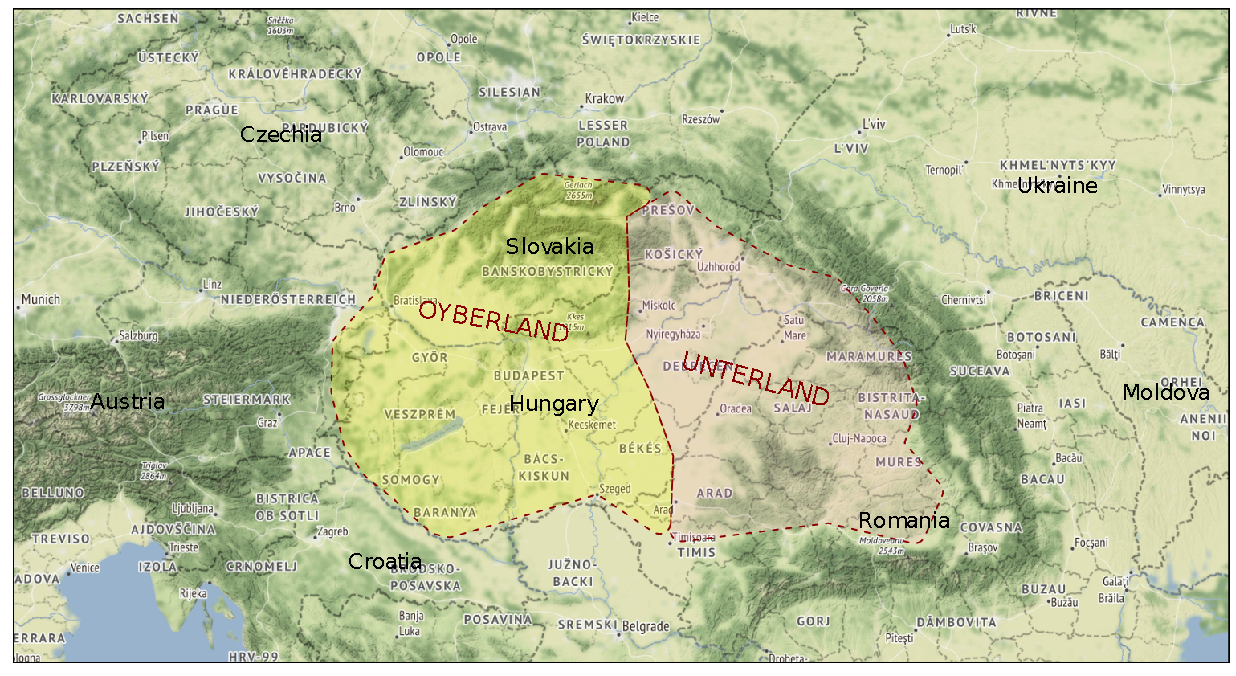
\includegraphics[width=\textwidth]{Fig1.Unterland_Oyberland.pdf}
\caption{\label{fig:nove:1} Present-day map showing the approximate boundaries of the historical Oyberland and Unterland regions based on demarcations by \citet{Krogh2012} and \citet{Weinreich1964}.}
\end{figure}

While not nearly as linguistically assimilated as the Oyberlender, Unterlender Jews were still somewhat less likely to be Yiddish dominant than their Polish brethren; and Unterlender women, who typically attended public school as children, were far more prone to linguistic assimilation than their male counterparts, most of whom received a religious education, in Yiddish (see e.g., \citealt[152]{Rubin1972}, \citealt[12]{Jelinek2007}).


In summary, if the Jewish communities of Central Poland can be regarded as emblematic of Eastern European Jewish culture by virtue of their longevity, geographical centrality, and size, the Unterland communities should be viewed as peripheral. Established relatively late in European Jewish history, they were somewhat insulated from other Jewish communities to the north and the east by the Carpathian Mountains that encircled them. Although the population grew rapidly in the nineteenth century, the number of Jews, even in the big cities of the region, remained low in comparison to Polish urban centers (\citealt[13]{Jelinek2007}). Moreover, the Unterland was, in many ways and for many people, a transitional place, a waystation, as \citet[34]{Jelinek2007} describes it:

\begin{quote}
[…] it appears that during the nineteenth century Subcarpathian Rus' [corresponding to the Zakarpattia Oblast in modern Ukraine] served, on the one hand, as a place of refuge for Jews from neighboring lands and, on the other, as a transit point for those who wanted to leave central Europe altogether. 
\end{quote}

Furthermore, Jewish communities in the Unterland were embedded within a larger multiethnic society and developed against a backdrop of shifting political borders and conflicting Jewish ideologies (\citealt{Keren-Kratz2019,Cooper2019,Jelinek2007,Švorc2020}; see also \citealt{Schäfer2022} on the influence of political boundaries on Yiddish dialects more generally.). Indeed, \citet[200]{Cooper2019} categorizes Carpathian Ruthenia, which is contained within the Unterland, as a borderland, and refers to it as a metaphorical ``catchbasin'' containing elements of Jewish ideologies ``collected'' from the surrounding regions. Linguistically, Unterland communities were in contact with a variety of co-territorial languages, including Hungarian, German, Romanian, Ukrainian, Ruthenian, Czech, and Slovak; and were in close contact with Oyberland communities, whose (Western) Yiddish dialect influenced their own (U. \citealt{Weinreich1964}). Finally, as noted above, there was a strong tendency among female Unterland speakers toward assimilation to the local majority language, usually Hungarian.

We believe that the circumstances described here make it highly likely that Unterland Central Yiddish diverged from Polish Central Yiddish and developed independently in the century preceding WWII and justify our view of Polish Yiddish as the more stable, conservative dialect and Unterland Yiddish as potentially innovative.

\subsection{Problems and hypotheses}
\label{sec:nove:3.3}

As noted above, initial research comparing data from interviews with New York–area speakers of Hasidic Yiddish and data from interviews with Holocaust survivors from the Hungarian Unterland revealed a surprisingly short duration distinction on the part of the latter for the vowels \mbox{/a/} and \mbox{/i/} -- below the 50 milliseconds proposed by \citet{LabovBaranowski2006} as the threshold for perceiving difference in vowels that differ primarily in length \citep{Nove2021}. Furthermore, the duration differences between the long and short vowels \mbox{/i/} and \mbox{/a/} of the female speakers in that study were significantly smaller than those of the males. Given the recurring trend in sociolinguistics for females to be at the forefront of change, and especially in light of the female tendency for linguistic assimilation in the Unterland, this result suggests that the shrinking differences reflect a change in progress.

The aim of this study is thus to further explore vowel length contrasts in Central Yiddish. The first goal was to replicate the findings by \citet{Nove2021} using a slightly expanded dataset of fifteen (versus twelve) speakers, eight of them female. The second and more important objective was to compare the duration differences in the Yiddish spoken in the Central Poland and Unterland regions in order to get a better idea of the nature of the length contrast in the vowel systems of these subdialects; and to discover whether there is evidence of divergence. Our prediction was that the duration differences in the vowels of Unterland speakers would be significantly smaller than those of the Central Poland speakers, with an effect of gender in the former group similar to the one found in the previous study.

\section{Data and methods}
\label{sec:nove:4}
The data for this project come from the newly developed \textit{Corpus of Spoken Yiddish in Europe} (CSYE), which is funded by the U.S. National Science Foundation under the supervision of Isaac Bleaman of the University of California, Berkeley \citep{BleamanNovePress}. The CSYE is an open-access digital language archive based on approximately two hundred interviews with Holocaust survivors, each of which averages about two hours in length, video-recorded by the \textit{USC Shoah Visual History Foundation} during the 1990s. The CSYE team is currently in the process of transcribing these interviews and reviewing the transcriptions, and testimonies are being published on a dedicated website (\href{http://yiddishcorpus.org/}{{yiddishcorpus.org}}) in audio and text formats when their transcripts are completed. The CSYE enabled us to create a corpus of the first hour of testimonies by fifteen speakers from the Unterland region (including nine that were part of \citet{Nove2021}, and eight speakers from Central Poland for analysis (\citealt{Archive2022a,Archive2022b}).\footnote{As of this writing, most of the testimonies analyzed in this study are pending final review prior to publication on the web site.} An additional benefit of this data source is the possibility of expanding the sample size as more testimonies are processed (\citealt{Nove2023,NoveSadock}). The present study is the first utilization of the data emerging from the project.

\subsection{Data processing}
\label{sec:nove:4.1}

Recordings in our corpus were transcribed in ELAN according to the protocols established by the CSYE by a team that includes both authors, and the transcriptions were reviewed. A pronunciation dictionary was created based on unique words in the corpus and was used to align the audio and text into word and sound segments using the Montreal Forced Aligner \textit{train and align} function \citep{McAuliffeEtAl2017}. Formant frequencies and duration measures were extracted from the sound files and TextGrids using a Praat plug-in called Fast Track \citep{Barreda2021}. 

The rest of the data processing, analysis, and visualization was conducted using R software (\citealt{Team2021}). The data were filtered to remove the most reduced function words and other reduced words. Mahalanobis distance was calculated by speaker for each vowel using the \texttt{tidy\_mahalanobis()} function in the \texttt{joeyr} package (an implementation of \texttt{mahalanobis()}) \citep{Stanley2020}, and the highest 5\% were discarded. The vowel midpoints (median taken from the 40--60\% vowel duration segment) were then normalized using the modified Nearey method utilized by Labov and colleagues in \textit{The Atlas of North American English} (\citealt{LabovBoberg2006}) via the \texttt{norm\_anae()} function in the \texttt{joeyr} package \citep{Stanley2020}, and the data were filtered to include only the target vowels.\footnote{One reviewer expressed a concern that survivors might have modified their speech in a way that would have impacted their vowels, at least in the very beginning of the interview, due to the perceived formality of the encounter. While some sociolinguists choose to discard the first five minutes of an interview for this very reason, we were loath to do so given that only the first hour of these interviews had been transcribed at the time and we did not want to lose any of the valuable data. Instead, we listened to the testimonies carefully and used our judgments about whether the speakers' dialects were typical for the location. While doing so, we identified one speaker (Robak) who used the more standard pronunciation [aɪ] in place of the expected CY form [a:]. For this reason, all tokens of the relevant long-short vowel pair by this speaker were excluded from our analysis. Other than the aforementioned issue with one particular speaker and a number of isolated instances of accommodation or interference of prestige forms, we did not encounter any systematic deviances that would skew the analyses.}

\begin{figure}
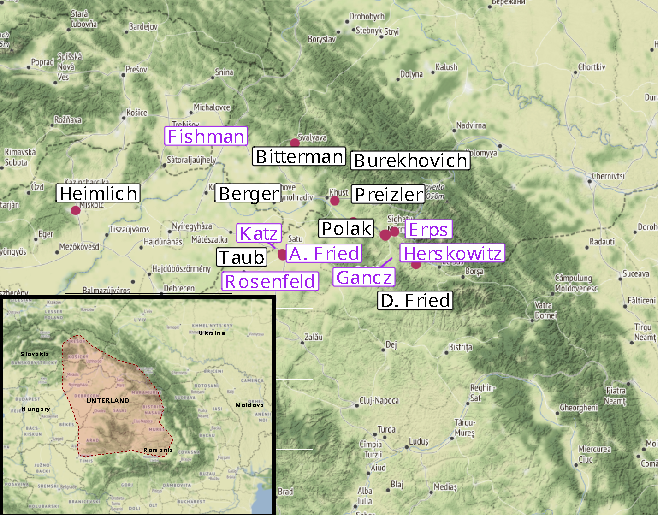
\includegraphics[width=.9\textwidth]{Fig2.Unterland_speakers_color.pdf}
% 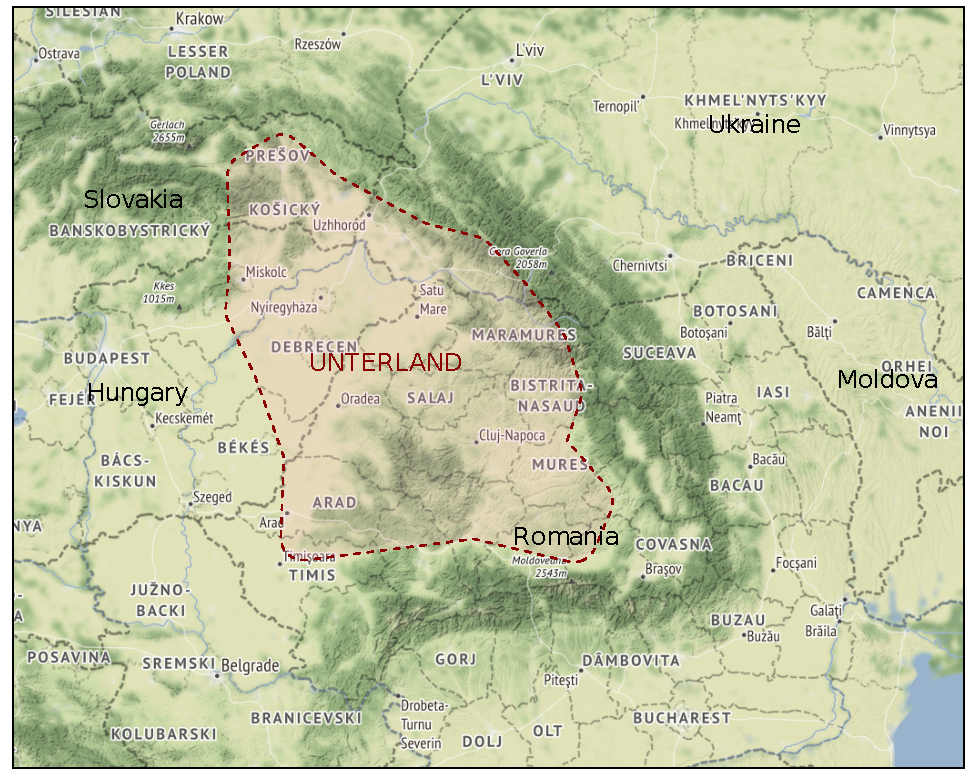
\includegraphics[width=.4\textwidth]{Fig2.inset.Unterland_bounds_broad.pdf}
\caption{\label{fig:nove:2}Map with points showing cities where fifteen Unterland speakers were raised and labels displaying the last names of female speakers in black text and male speakers in purple. Insert map delineates the approximate boundaries of the Unterland within the larger region.}
\end{figure}


Two analyses were conducted using this data output. The first, designed to replicate the results of \citet{Nove2021}, calculated the duration differences in the vowels of fifteen Unterland speakers, eight of them female, and checked for a gender effect. \tabref{tab:nove:1} shows a list of the fifteen Unterland speakers by last name, birth year, gender, and the locations (city and country) in which they were raised; these locations are shown on the map in \figref{fig:nove:2}.\footnote{Note: Name label positions on the map are shifted slightly to avoid overlap.}

\begin{table}
\small
\begin{tabular}{llclll}
    \lsptoprule
    & Birth &           & City Raised &             & Interview\\
    {Speaker} & {Year} & {Gender} & {(Yiddish)} & {Presently} & {Country}\\
    \midrule
    Berger & 1925 & F & Beregsaz & Berehovo, UA & Israel\\
    Bitterman & 1923 & F & Svalyeve & Svaliava, UA & U.S.\\
    Burekhovich & 1920 & F & Boronyave & Boronyava, UA & U.S.\\
    Erps & 1922 & M & Kretshenif & Crăciunești, RO & U.S.\\
    Fishman & 1919 & M & Ungvar & Užhorod, UA & Israel\\
    A. Fried & 1917 & M & Satmar & Satu Mare, RO & Israel\\
    D. Fried & 1913 & F & Rezavlye & Rozavlea, RO & U.S.\\
    Gancz & 1924 & M & Siget & Sighetu Marmaţiei, RO & Sweden\\
    Heimlich & 1925 & F & Mishkolts & Miskolc, HU & Australia\\
    Herskowitz & 1922 & M & Siget &  & U.S.\\
    Katz & 1924 & M & Satmar &  & U.S.\\
    Polak & 1922 & F & Tetsh & Tyachiv, Ukraine & Australia\\
    Preizler & 1914 & F & Siget &  & Israel\\
    Rosenfeld & 1910 & M & Satmar &  & Canada\\
    Taub & 1911 & F & Satmar &  & Israel\\
    \lspbottomrule
\end{tabular}
\caption{\label{tab:nove:1}Fifteen Unterland speakers by last name, birth year, gender, location in which they were raised, and country in which they were interviewed.}
\end{table}
  

The objective for the second analysis was to test the hypothesis in \citet{Nove2021} about subdialectal divergence within CY across these two regions. To this end, we compared male speakers raised in interwar Central Poland (Warsaw and nearby areas) and the Unterland. In this comparative analysis, we only included the male speakers from the Unterland for consistency (since we did not yet have any data from Polish females to analyze). \tabref{tab:nove:2} shows a list of the six Polish speakers and \figref{fig:nove:3} shows their respective places of origin.

\begin{table}
\begin{tabular}{llclll}
\lsptoprule
          & Birth  &          & City     &             & Interview\\
{Speaker} & {Year} & {Gender} & {Raised} & {Presently} & {Country}\\
\midrule
Popowski & 1918 & M & Varshe & Warsaw, PL & Argentina\\
Robak & 1922 & M & Varshe &  & Poland\\
Sherman & 1925 & M & Apt & Opatów, PL & Israel\\
Silver & 1911 & M & Varshe &  & Australia\\
Scheinberg & 1912 & M & Varshe &  & U.S.\\
Zylberberg & 1922 & M & Varshe &  & Argentina\\
\lspbottomrule
\end{tabular}
\caption{\label{tab:nove:2} Six Polish speakers by last name, birth year, gender, location in which they were raised, and country in which they were interviewed.}
\end{table}
  
\begin{figure}
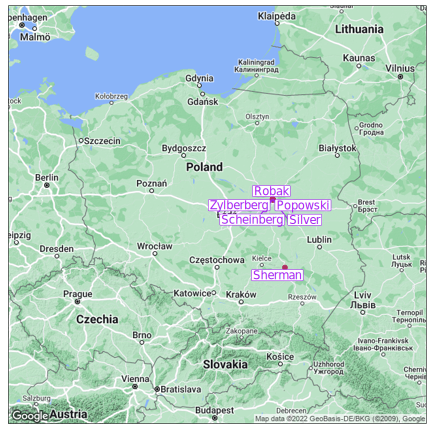
\includegraphics[width=\textwidth]{Fig3.Poland_speakers_color.png}
\caption{\label{fig:nove:3} Map with points showing cities where the six Polish speakers were raised and labels displaying the speakers' last names.}
\end{figure}

Using the methodology described here, we extracted a total of 27,163 vowels, 19,864 from the Unterland and 7,299 from Central Poland, for analysis. \tabref{tab:nove:3} and \tabref{tab:nove:4} show the breakdown of vowels analyzed in each class for each subregion.

\begin{table}
\captionsetup{margin=.05\linewidth}
\begin{floatrow}
\ttabbox{\begin{tabular}{lrr}
\lsptoprule
{vowel} & {count} & {\% of sub corpus}\\
\midrule
iː & 2552 & 0.13\\
i & 4806 & 0.24\\
uː & 2316 & 0.12\\
u & 2118 & 0.11\\
aː & 1686 & 0.08\\
a & 6386 & 0.32\\
\lspbottomrule
\end{tabular}}
{\caption{\label{tab:nove:3} Breakdown of Unterland vowels analyzed by vowel category.}}
\ttabbox{%
\begin{tabular}{lrr}
\lsptoprule
{vowel} & {count} & {\% of sub corpus}\\
\midrule
iː & 1003 & 0.14\\
i & 1744 & 0.24\\
uː & 775 & 0.11\\
u & 667 & 0.09\\
aː & 766 & 0.10\\
a & 2344 & 0.32\\
\lspbottomrule
\end{tabular}}
{\caption{\label{tab:nove:4} Breakdown of Central Poland vowels analyzed by vowel category.}}
\end{floatrow}
\end{table}

\subsection{Statistical analysis}
\label{sec:nove:4.2}

To test for differences across genders and regional groups, linear mixed-effects regression models were fit for each pair of vowels using the \texttt{lmer()} function in the \texttt{lme4} package \citep{BatesEtAl2013}. The Satterthwaite approximation in the \texttt{lmerTest} package (\citealt{KuznetsovaChristensen2017}) was used to calculate all \textit{p}-values. Each model had decadic log of vowel duration as the dependent variable and included the following variables and interactions as fixed effects:

\begin{enumerate}
\item  Interaction: vowel × gender (Unterland only)
\item  Interaction: vowel × corpus
\item  Number of segments in the word
\item  Preceding segment (silence, vowel, or consonant coded for voice, manner, and place of articulation)
\item  Following segment (silence, vowel, or consonant coded for voice, manner, and place of articulation)
\item  Interview country (to infer influence of postwar contact language)
\end{enumerate}

Random intercepts:

\begin{enumerate}
\item[7.] Speaker
\item[8.] Word
\end{enumerate}

To quantify the relative overlap between vowel pairs on the quality dimension, we grouped the data by gender and region and performed a MANOVA, with F1 and F2 as the dependent variables and vowel, phonological context, and duration as independent variables, generating a Pillai score for each pair (\citealt{HayDrager2006, NyczHall-Lew2013}). The MANOVA output also includes a \textit{p}-value for the Pillai score that indicates whether the difference between the two vowel clusters is significant.

\section{Results}
\label{sec:nove:5}
\subsection{Unterland}
\label{sec:nove:5.1}
\subsubsection{Vowel duration}
\label{sec:nove:5.1.1}

The results of the Unterland analysis replicate the findings of \citet{Nove2021} in that the duration differences of all vowel pairs are remarkably small. \figref{fig:nove:4} shows mean vowel duration (in milliseconds) for all Unterland speakers, calculated separately by gender group and labeled with the mean difference for each pair. Female speakers also exhibit smaller differences for \mbox{/i/} and \mbox{/a/} than their male counterparts, and their differences fall below 50 milliseconds for all vowel pairs.

  \largerpage
\begin{figure}
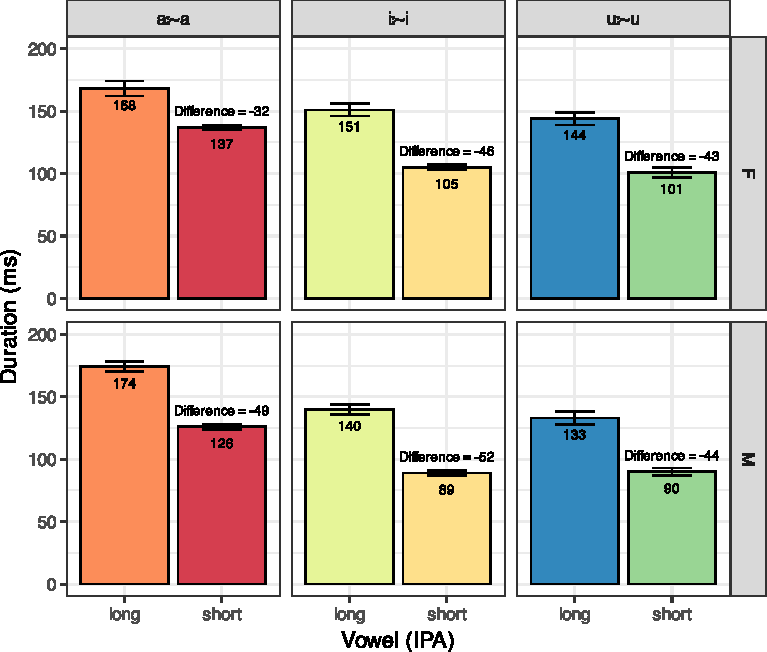
\includegraphics[width=.9\textwidth]{Fig4.plot_dur_bars.Unt.gend}
\caption{\label{fig:nove:4}Unterland mean duration faceted by vowel pair (columns) and by gender (rows), with 95\% confidence interval standard error bars. Annotations on the bars indicate mean duration for each vowel, and the durational differences between the vowels in each pair are shown above the short vowel bar.}
\end{figure}

Regression analyses (LMM) indicate that these differences are statistically significant: the models for duration show a significant effect of gender in \mbox{/i/} and \mbox{/a/}. In \figref{fig:nove:5} the gender differences can be seen in the different slopes of the lines on plots of estimated means extracted from the regression models, with vowel on the x-axis and duration on the y-axis.\footnote{The reason why the female speakers in this study have longer vowel durations overall is probably because several of the female speakers have particularly slow speech rates.} The results of the LMMs are shown in the appendix (\sectref{sec:nove:AppendixA}).

\begin{figure}
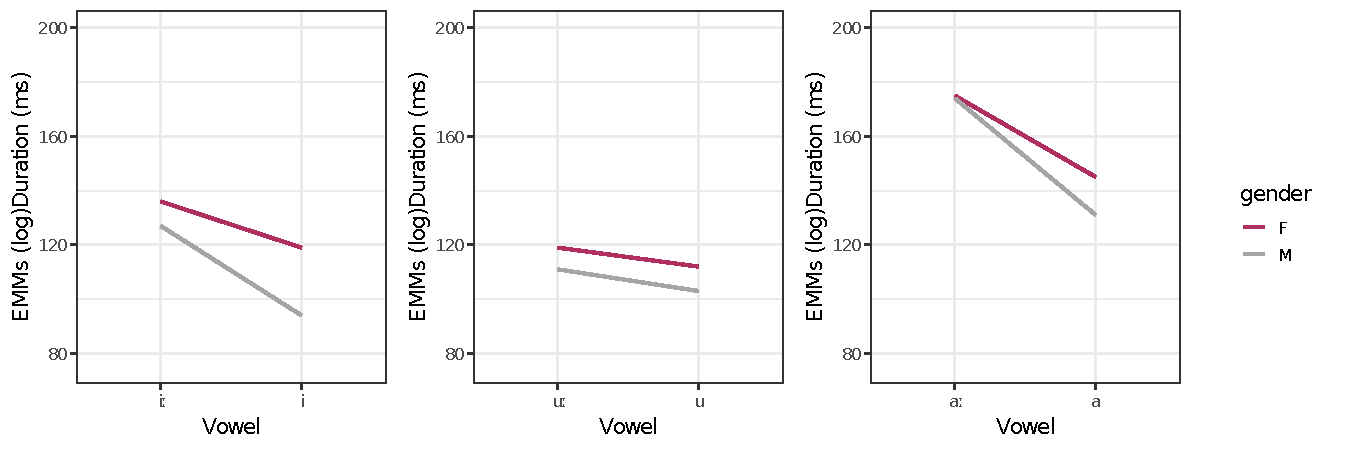
\includegraphics[width=.9\textwidth]{Fig5.plot_emmeans.UNT.dur.pdf}
\caption{\label{fig:nove:5} Unterland estimated marginal means of duration LMM for all vowel pairs, with vowel on the x-axis and duration (back-transformed from decadic log) on the y-axis, faceted by gender (rows), with lines connecting the vowels, colored by gender group.}
\end{figure}

\subsubsection{Vowel quality}
\label{sec:nove:5.1.2}

Our analysis of vowel quality among Unterland speakers did not yield any informative patterns thus far. \figref{fig:nove:6} is a contour plot of F1 and F2 values, faceted by gender, in which the lines represent density of the data. Among the female speakers there appears to be more lowering of [i] relative to [iː], but the short vowels of both pairs are more centralized among the male speakers. (Note that the bimodal distribution in the male \mbox{/a/} is caused by one outlier speaker whose vowel space is particularly small, hence the higher \mbox{/a/s}.)

\begin{figure}
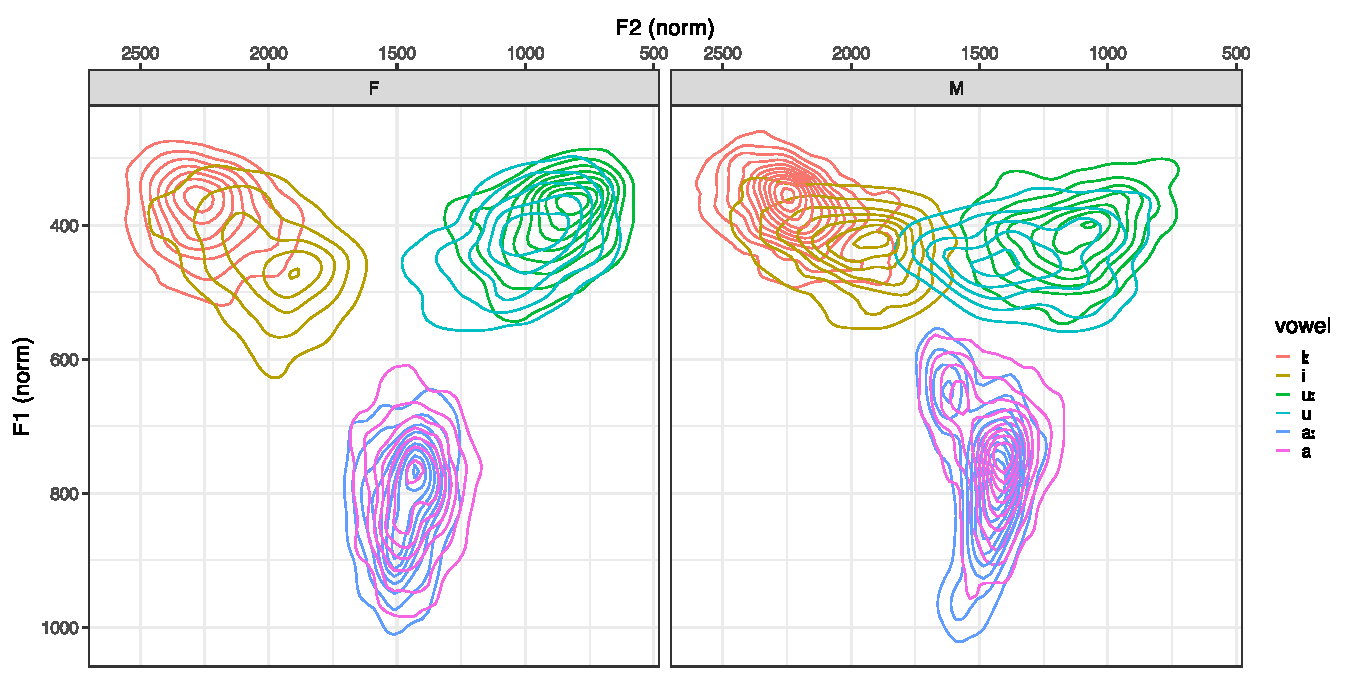
\includegraphics[width=\textwidth]{Fig6.contour.Unterland_by.gender.pdf}
\caption{\label{fig:nove:6}Contour plots of all vowel tokens (N = 19,864) by Unterland speakers by F1 and F2 and density, faceted by gender group.}
\end{figure}

The results of the MANOVAs are in \tabref{tab:nove:5}. Pillai scores range from 0 to 1, with 1 indicating no similarity between the two clusters and 0 indicating no difference. Based on these scores, the quality of the long and short vowels in the high vowel pairs are similar, and they are nearly identical in \mbox{/a/}. Female speakers appear to be more merged in all vowel pairs than males; however, the differences between uː{\textasciitilde}u and aː{\textasciitilde}a are minimal.

\begin{table}
\begin{tabularx}{.8\textwidth}{XXrr}
\lsptoprule
{ vowel} & { gender} & { Pillai} & { $p$-value}\\
\midrule
iː{\textasciitilde}i & F & 0.203 & 0.000\\
& M & 0.313 & 0.000\\
\midrule
uː{\textasciitilde}u & F & 0.096 & 0.000\\
& M & 0.169 & 0.000\\
\midrule
aː{\textasciitilde}a & F & 0.012 & 0.000\\
& M & 0.049 & 0.000\\
\lspbottomrule
\end{tabularx}
\caption{\label{tab:nove:5} Pillai scores derived from a MANOVA measuring spectral overlap for all vowel pairs by gender group.}
\end{table}

In examining the data, we noted a great deal of interspeaker variability in the spectral overlap of the long-short high vowels in both gender groups. This is reflected in by-speaker Pillai scores (not shown here), which show a wide range within each group. However, we did not find a correlation between by-speaker Pillai scores and duration difference in these vowel pairs.

To illustrate the kind of interspeaker variability we observed, we present \figref{fig:nove:7}, which plots the peripheral vowels of the most and the least merged speakers in our dataset by F1 and F2. The most merged speaker (Taub, on the right) happens to be female, and the one with the most separation (Herskowitz, on the left) is male. Their Pillai scores are shown in \tabref{tab:nove:6}.


\begin{figure}[t]
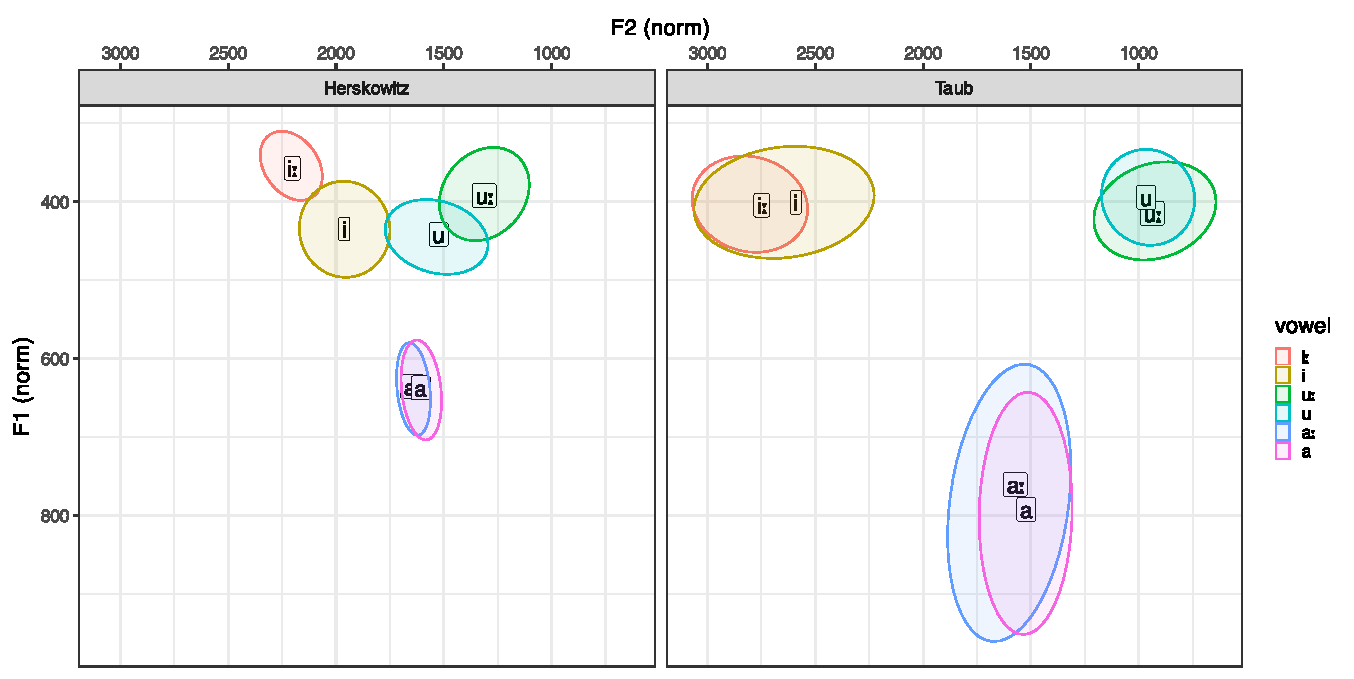
\includegraphics[width=\textwidth]{Fig7.vowel_plot_ellips.2speakers.pdf}
\caption{\label{fig:nove:7} Vowel tokens (N = 2,472) of two speakers (Herskowitz, M and Taub, F) plotted by F2 on the x-axis and F1 on the y-axis. Square labels containing IPA symbols represent the location of the vowel means, and ellipses show 68\% confidence in the mean.}
\end{figure}

\begin{table}
\begin{tabularx}{.8\textwidth}{XXrr}
\lsptoprule
{ speaker} & { vowel} & { Pillai} & { $p$-value}\\
\midrule
Herskowitz & iː{\textasciitilde}i & 0.584 & 0.000\\
& uː{\textasciitilde}u & 0.498 & 0.000\\
& aː{\textasciitilde}a & 0.065 & 0.000\\
\midrule
Taub & iː{\textasciitilde}i & 0.059 & 0.001\\
& uː{\textasciitilde}u & 0.064 & 0.012\\
& aː{\textasciitilde}a & 0.028 & 0.013\\
\lspbottomrule
\end{tabularx}
\caption{\label{tab:nove:6} Pillai scores derived from a MANOVA measuring spectral overlap for all vowel pairs by two speakers for all vowel pairs.}
\end{table}

It also happens that Mrs. Taub immigrated to Israel after the war and Mr. Herskowitz resettled in the United States. Recall that these interviews were conducted about fifty years after the war, and that these two speakers are now (presumably) also speakers of Israeli Hebrew and American English, respectively. Note also the similarity between Herskowitz's vowel system and the English tense-lax system in the high vowels. Modern Hebrew, on the other hand, has no contrast in these vowels. There is ample evidence in the literature on second language acquisition that even minimal experience with an L2 can influence a speaker's L1 (e.g., \citealt{Chang2011}). While this analysis has revealed nothing definitive regarding vowel quality thus far, an expanded dataset and more detailed analyses, including an analysis of vowel trajectories rather than just the midpoint measures, might reveal additional patterns of variation.

\subsection{Central Poland}
\label{sec:nove:5.2}
\subsubsection{Vowel duration}
\label{sec:nove:5.2.1}
We turn now to the second aim of our study, a comparison of the durational distinctions in Unterland and Polish CY vowel pairs. Looking at the mean duration with long-short differences by corpus (\figref{fig:nove:8}), we can immediately see larger differences in the high vowels of the Polish speakers, but not in \mbox{/a/}.

  
\begin{figure}[t]
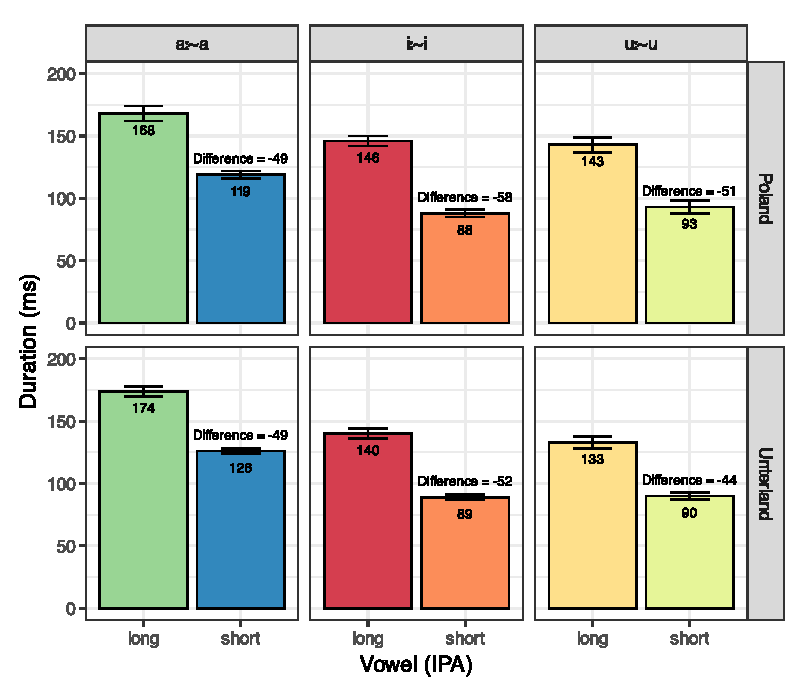
\includegraphics[height=.5\textheight]{Fig8.plot_dur_bars.corp.pdf}
\caption{\label{fig:nove:8} Mean duration for male speakers faceted by vowel pair (columns) and by sub corpus (rows), with 95\% confidence interval standard error bars. Annotations on the bars indicate mean duration for each vowel and the durational differences between the vowels in each pair are shown above the short vowel bar.}
\end{figure}

\begin{figure}[b]
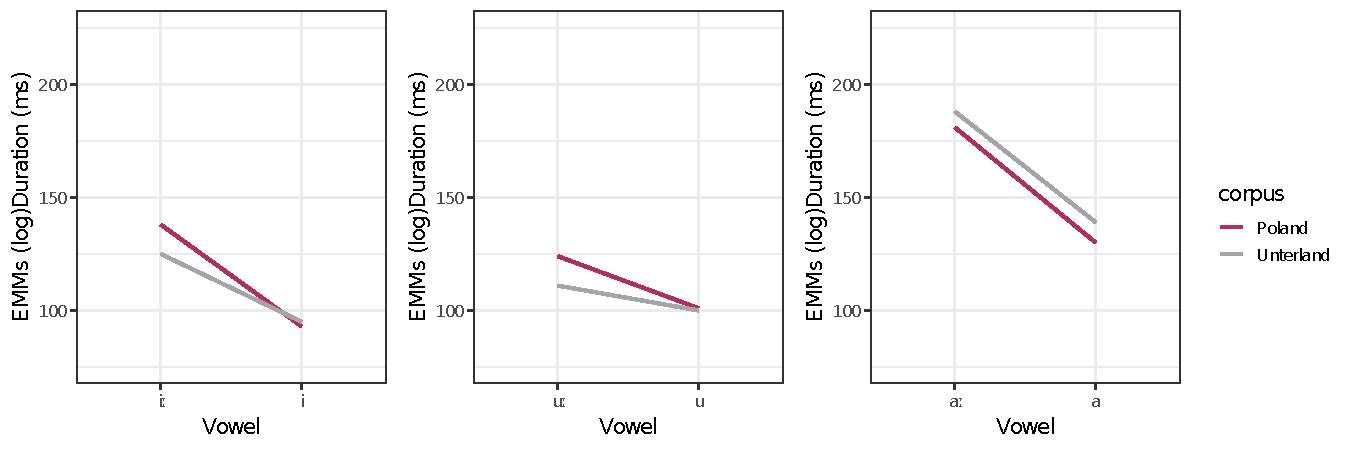
\includegraphics[width=\textwidth]{Fig9.plot_emmeans.CORP.dur_ALT.pdf}
\caption{\label{fig:nove:9} Estimated marginal means of duration LMM, with vowel (long vs. short) on the x-axis and duration (back-transformed from decadic log) on the y-axis, faceted by vowel pair, with lines connecting the vowels colored by corpus (Poland vs. Unterland).}
\end{figure}

Regression modeling indicates that these variances are statistically significant. That is, the models for duration show a significant effect of region in the \mbox{/i/} and \mbox{/u/} pair. These differences can be seen by examining the slopes on the plots below (\figref{fig:nove:9}), which show estimated means of duration by vowel for each pair, with lines connecting the long-short vowels colored by regional group. The results of the LMMs are shown in the appendix.

\clearpage

\subsubsection{Vowel quality}
\label{sec:nove:5.2.2}

Comparing the two regions on the quality dimension, we once again find our results do not account for the results obtained for vowel duration. A vowel plot of all male speakers, faceted by regional group, is shown in \figref{fig:nove:10}. Here too there appears to be a substantial amount of interspeaker variability in the amount of spectral overlap of the long-short vowels in the high vowel pairs within each group. While the high front vowels look a bit more separated in the Polish corpus, the high back vowels appear more separated in the Unterland corpus. Pillai scores calculated for each region, shown in the \tabref{tab:nove:7}, suggest that these differences are indeed very small.

\begin{figure}
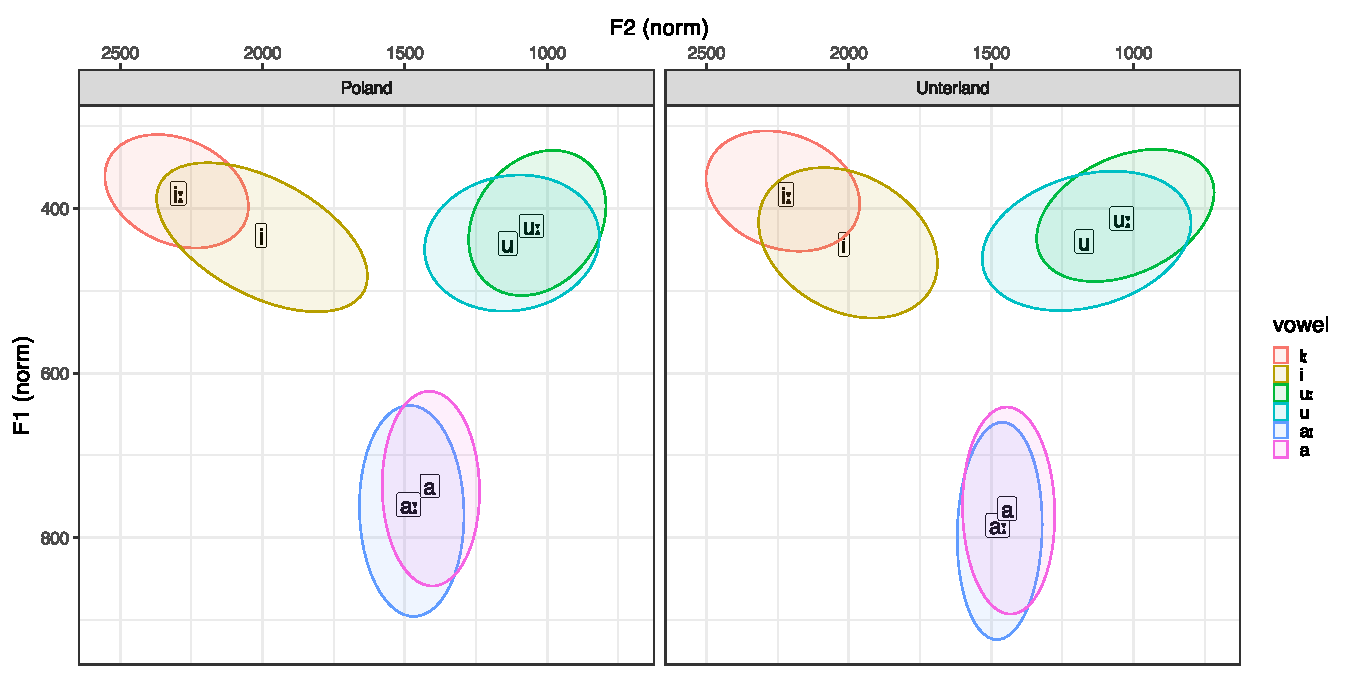
\includegraphics[width=\textwidth]{Fig10.vowel_plot_ellips.corpus.pdf}
\caption{\label{fig:nove:10} Vowel tokens (N = 17,405) of all male speakers plotted by F2 on the x-axis and F1 on the y-axis, faceted by regional group (Poland vs. Unterland). Square labels containing IPA symbols represent the location of the vowel means, and ellipses show 98\% confidence in the mean.}
\end{figure}

\begin{table}
\begin{tabularx}{.8\textwidth}{XXrr}
\lsptoprule
{ corpus} & { vowel} & { Pillai} & { $p$-value}\\
\midrule
Poland & iː{\textasciitilde}i & 0.325 & 0.000\\
& uː{\textasciitilde}u & 0.073 & 0.000\\
& aː{\textasciitilde}a & 0.073 & 0.000\\
Unterland & iː{\textasciitilde}i & 0.241 & 0.000\\
& uː{\textasciitilde}u & 0.101 & 0.000\\
& aː{\textasciitilde}a & 0.021 & 0.000\\
\lspbottomrule
\end{tabularx}
\caption{\label{tab:nove:7} Pillai scores Pillai scores derived from a MANOVA measuring spectral overlap of male speaker for all vowel pairs by regional group (Poland vs. Unterland).}
\end{table}

It is important to note that in this study we did not analyze a phonological process that reportedly affects the quality of a subset of the target vowels: the insertion of epenthetic schwa between certain long vowels and particular coda consonants.\footnote{\citet{Jacobs1993} proposes that such vowel diphthongization is motivated by a phonological avoidance of syllable overlength and formulates two separate but related phonological rules, which he calls \textit{breaking} and \textit{drawl}, to describe the process. \citet{Garellek2020}, however, treats it as a single phenomenon and offers a phonetic explanation for the occurrence or nonoccurrence of schwa insertion in such contexts.}  Previous analyses by \citet{Nove2021}, and our own impressions from the data, suggest that the absence or presence of this conditioned diphthongization varies greatly across the CY dialect region. Thus, a careful comparison of vowel quality in these two regions may require that the entire trajectory of the vowels, not merely their midpoints, be analyzed. Plans are underway to conduct such a study on an expanded dataset. We thus refrain from positing anything definitive about vowel quality pending the completion of that analysis. 

\section{Discussion}
\label{sec:nove:6}
In this study we analyzed the acoustic correlates of an historical length contrast in CY across two dialect regions: Central Poland and the Unterland. We discovered significant differences in duration distinction across gender groups within the Unterland (in \mbox{/i/} and \mbox{/a/}), and among male speakers across regional groups (in \mbox{/i/} and \mbox{/u/}). The results provide some tentative answers to the research questions that motivated this study and give rise to several others. 

The small durational differences found in the long-short vowel pairs of speakers in the Unterland region, with females exhibiting significantly shorter differences than males, suggest a change in progress with females in the lead, consistent with the oft-observed trend for female speakers to lead in linguistic innovation. That the Polish (male) speakers have significantly larger durational differences than the Unterlender (male) speakers reinforces this interpretation, especially when considering the relative recency of the establishment of Unterland Jewish communities versus the long and continuous presence of Jews in Central Poland. Taking into consideration other circumstantial factors, including the mountainous barrier between Poland and the Unterland and the degree of multilingualism, linguistic assimilation, and geopolitical turmoil in the latter region, we seem to have the optimal conditions for linguistic innovation and dialect divergence. 

Thus far we do not have an explanation for why this feature was affected and why in this particular direction. Another puzzle is the fact that while the gender effect shows up in the \mbox{/i/} and \mbox{/a/} pairs in the Unterland, the regional differences are in the \mbox{/i/} and \mbox{/u/} pairs. There is a substantial amount of interspeaker variation in the duration of \mbox{/u/} among Unterland speakers, which may account for the lack of gender effect there. On the other hand, as noted above, \mbox{/u/} differs from the other two vowels in that the contrast is not an inherited feature of proto\hyp Yiddish but came about through a more recent split conditioned by phonological environment. Indeed, although it is treated as a length distinction in most of the literature, the phonemic status of short \mbox{/u/} is disputed by some (e.g., \citealt{Beider2015}). We believe that the different behavior of \mbox{/u/} compared to the other two vowel pairs is related to its non-phonemic status, and we are currently experimenting with other methods to further explore these differences. As for the absence of a regional effect in \mbox{/a/}, it is possible that Unterland males have simply not yet reached the threshold of significance. Additionally, \mbox{/a/} is different from \mbox{/i/} and \mbox{/u/} in one very important respect: the contrast is represented orthographically. There is also a strong mental awareness of the diphthongal origin of \mbox{/aː/}, and it is not uncommon for speakers to pronounce it as a diphthong in read or formal speech. Moreover, the dialects that have \mbox{/aɪ/} for this vowel (primarily NEY) are considered more prestigious. In fact, one of the speakers in our Polish corpus had to be excluded from the analysis of \mbox{/a/} because he often pronounces long \mbox{/a/} as [aɪ]. So it is likely that the higher rate of literacy among Yiddish\hyp speaking males in that era had the effect of preserving the contrast in \mbox{/a/} to some extent, accounting for this effect.

\section{Conclusions}

A desideratum of \citet{SadockMasor2018} was a better understanding of intradialectal differences within the CY dialect region. Our finding of differences in durational distinctions between the Central Poland and Unterland regions is a definitive step in that direction. We are currently working on an expanded version of this study, which includes female speakers from Central Poland, to shed more light on the gender patterns within and across both regional groups. We are also hoping to eventually broaden the geographic reach of this study farther into Poland, and especially into Galicia,\footnote{Most of Galicia is within CY territory, although the easternmost region of it, including Kilemey and Tarnepol (Kolomyya and Ternopil' in Ukraine) is usually grouped with SEY because of the realization of the reflex of MHG \textit{ei} as \mbox{/ej/}, not \mbox{/aj/} there.}  the region immediately to the north of the Unterland, across the Carpathians. In addition to vowel length, we have plans to analyze other phonetic features, such as presence or absence of vowel breaking, differences in \mbox{/l/} and \mbox{/r/} quality, and postvocalic \mbox{/r/} deletion. 

It must be noted that the data from the CSYE, while extremely rich in a variety of ways, also inherently contain some limitations for linguistic analysis. For one, at the time of the interviews, nearly all the speakers had spent decades living far away from the cities and towns in which they grew up and had presumably acquired the language of their host country to some extent. It is well known that language can change across a person's lifespan and that exposure to new languages can influence a speaker's first language. Additionally, the interviewers themselves spoke a variety of dialects, often markedly non-natively, and it is impossible to assess what effect, if any, this had on the survivors' speech. Nevertheless, given that the Holocaust effectively destroyed the Yiddish\hyp speaking communities of Eastern Europe, these interviews constitute the best available corpus of high-quality recordings of people who grew up in prewar European Yiddish\hyp speaking communities.

Yiddish is one of very few Germanic dialects that have not been subjected to systematic acoustic analyses, which is unfortunate, given that careful classification of its dialects depends on knowledge of their phonological features. While the destruction of the European Yiddish\hyp speaking homeland certainly complicates such endeavors, this study illustrates how archival recordings can be used to evaluate previous claims about Yiddish dialects and discover additional nuance within and among them. The CSYE will be, upon completion, a source not merely of a large amount of high-quality data suitable for acoustic analysis but also of data from speakers in areas that have previously not been studied, especially marginal and transitional dialect regions. 

Finally, but perhaps most importantly, this comparative study functions as an important link between the Yiddish of today and that of the prewar era, making it possible to evaluate claims about linguistic innovation in contemporary Yiddish vowels. As such, it fills an important gap in Yiddish linguistics. Indeed, in a study comparing the peripheral vowels of three generations of contemporary Hasidic Yiddish speakers in New York, \citet{Nove2021} uses data from this archive as a baseline and finds that among the first New York-born generation, the durational differences actually increased in the high vowels relative to the immigrant generation – an apparent reinforcement of a tenuous contrast. Among subsequent generations, however, Nove observes a gradual shift in the quality of the short high vowels, with the youngest generation exhibiting a clear qualitative (tense-lax) contrast in these vowel pairs similar to the English (u{\textasciitilde}ʊ, i{\textasciitilde}ɪ). This study illustrates how careful studies of prewar Yiddish dialects can shed light on the interplay between the internal and external forces that drive language change. The observed changes in the Hasidic Yiddish vowel system reflect both the persistence of inherited linguistic features and the way that the language is adapting to a changing sociolinguistic context. Such insights are valuable not only for Yiddish linguistics but for a broader understanding of how minority diaspora languages develop in new language contact environments.




%\appendix
\section*{Appendix} %A: Results of Linear Mixed Models for the three vowel pairs of the Unterland speakers
\label{sec:nove:AppendixA}

%Some text to check whether the command works in general. Yes it does, so the size of the tables needs to be adapted to allow the headings to be printed, too, or we need to work with longtables …
%\todo[inline]{because the tables in the appendix are too long to fit the section heading onto the same page, I think we need to work with longtables here …}

{%%%\small
\begin{longtable}{l S[table-format=-1.2] S[table-format=1.2] S[table-format=-1.2] S[table-format=<1.3]}
\caption{Results of linear mixed model assessing durational distinction for the high vowels [iː] and [i] in the Unterland}\\
\lsptoprule
& \multicolumn{4}{c}{Duration (ms)}\\\cmidrule(lr){2-5}
Predictors & {Est.} & {SE} & {$t$} & {$p$} \\\midrule
\endfirsthead

\midrule 
& \multicolumn{4}{c}{Duration (ms)}\\\cmidrule{2-5}
Predictors & {Est.} & {SE} & {$t$} & {$p$} \\ \midrule
\endhead

\midrule \multicolumn{3}{r}{{Continued on next page}} \\ \midrule
\endfoot

\lspbottomrule
\endlastfoot


%\lsptoprule
%\midrule
(Intercept) & 2.20 & 0.05 & 45.95 & \bfseries <0.001\\
vowel IPA [i] & -0.06 & 0.01 & -5.11 & \bfseries <0.001\\
gender [M] & -0.03 & 0.04 & -0.75 & 0.455\\
num seg & -0.01 & 0.00 & -5.69 & \bfseries <0.001\\
pre context [corNAS] & -0.04 & 0.02 & -2.17 & \bfseries 0.030\\
pre context [dorGLI] & -0.15 & 0.03 & -5.43 & \bfseries <0.001\\
pre context [dorLIQ] & 0.01 & 0.14 & 0.06 & 0.950\\
pre context [labNAS] & -0.06 & 0.02 & -2.94 & \bfseries 0.003\\
pre context [UNK] & 0.01 & 0.02 & 0.66 & 0.511\\
pre context [V] & -0.09 & 0.03 & -3.54 & \bfseries <0.001\\
pre context [VcorOBS] & -0.01 & 0.02 & -0.49 & 0.621\\
pre context [VdorOBS] & -0.11 & 0.03 & -3.29 & \bfseries 0.001\\
pre context [VlabOBS] & -0.06 & 0.02 & -3.54 & \bfseries <0.001\\
pre context [XVcorOBS] & -0.10 & 0.01 & -7.78 & \bfseries <0.001\\
pre context [XVdorOBS] & -0.12 & 0.02 & -5.93 & \bfseries <0.001\\
pre context [XVlabOBS] & -0.12 & 0.02 & -6.44 & \bfseries <0.001\\
pre context [XVlarOBS] & 0.07 & 0.02 & 2.88 & \bfseries 0.004\\
post context [corLIQ] & 0.12 & 0.02 & 7.82 & \bfseries <0.001\\
post context [corNAS] & -0.09 & 0.02 & -5.43 & \bfseries <0.001\\
post context [dorGLI] & 0.06 & 0.12 & 0.55 & 0.583\\
post context [dorNAS] & -0.08 & 0.02 & -3.57 & \bfseries <0.001\\
post context [labNAS] & -0.10 & 0.02 & -4.73 & \bfseries <0.001\\
post context [UNK] & 0.26 & 0.03 & 7.43 & \bfseries <0.001\\
post context [V] & 0.06 & 0.03 & 1.82 & 0.068\\
post context [VcorOBS] & -0.02 & 0.02 & -1.24 & 0.214\\
post context [VdorOBS] & -0.04 & 0.02 & -1.79 & 0.074\\
post context [VlabOBS] & 0.10 & 0.02 & 5.41 & \bfseries <0.001\\
post context [XVdorOBS] & 0.02 & 0.02 & 1.26 & 0.209\\
post context [XVlabOBS] & -0.04 & 0.03 & -1.46 & 0.145\\
post context [XVlarOBS] & 0.08 & 0.05 & 1.58 & 0.115\\
country interview [Canada] & 0.02 & 0.08 & 0.19 & 0.853\\
country interview [Israel] & 0.07 & 0.05 & 1.32 & 0.186\\
country interview [Sweden] & 0.03 & 0.08 & 0.37 & 0.710\\
country interview [U.S.A.] & 0.01 & 0.05 & 0.14 & 0.886\\
vowel IPA [i] × gender [M] & -0.08 & 0.01 & -8.02 & \bfseries <0.001\\
\midrule
\multicolumn{5}{c}{Random Effects}\\
\midrule
σ\textsuperscript{2} & 0.03 & & & \\
τ\textsubscript{00} \textsubscript{word} & 0.01 & & &\\
τ\textsubscript{00} \textsubscript{speaker} & 0.00 & & &\\
ICC & 0.25 & & &\\
N \textsubscript{speaker} & 15 & & &\\
N \textsubscript{word} & 1054 & & &\\
\midrule
Observations & 7358 & & &\\
Marginal R\textsuperscript{2} & 0.283 & & &\\
Conditional R\textsuperscript{2} & 0.462 \\
\end{longtable}


%ALTE TABELLEN gelöscht

%\section*{\label{sec:nove:AppendixB}Appendix B}
\begin{longtable}{l S[table-format=-1.2] S[table-format=1.2] S[table-format=-1.2] S[table-format=<1.3]}
\caption{Results of linear mixed model assessing durational distinction for the high vowels [uː] and [u] in the Unterland}\\
\lsptoprule
 & \multicolumn{4}{c}{Duration (ms)}\\\cmidrule{2-5}
Predictors & {Est.} & {SE} & $t$ & {$p$} \\ \midrule
\endfirsthead

\midrule
& \multicolumn{4}{c}{Duration (ms)}\\
\cmidrule{2-5}
Predictors & {Est.} & {SE} & $t$ & {$p$} \\ \midrule
\endhead

\midrule \multicolumn{3}{r}{{Continued on next page}} \\ \midrule
\endfoot

\lspbottomrule
\endlastfoot

%\midrule
(Intercept) & 2.30 & 0.06 & 37.09 & \bfseries <0.001\\
vowel IPA [u] & -0.03 & 0.02 & -1.19 & 0.236\\
gender [M] & -0.03 & 0.05 & -0.71 & 0.476\\
num seg & -0.02 & 0.00 & -4.48 & \bfseries <0.001\\
pre context [corNAS] & -0.05 & 0.02 & -2.21 & \bfseries 0.027\\
pre context [dorGLI] & -0.18 & 0.05 & -3.40 & \bfseries 0.001\\
pre context [dorLIQ] & 0.02 & 0.11 & 0.21 & 0.835\\
pre context [labNAS] & -0.15 & 0.04 & -3.64 & \bfseries <0.001\\
pre context [OTHER] & -0.28 & 0.07 & -3.81 & \bfseries <0.001\\
pre context [UNK] & 0.03 & 0.03 & 1.20 & 0.230\\
pre context [V] & -0.01 & 0.03 & -0.33 & 0.743\\
pre context [VcorOBS] & -0.08 & 0.03 & -2.85 & \bfseries 0.004\\
pre context [VdorOBS] & -0.10 & 0.06 & -1.77 & 0.078\\
pre context [VlabOBS] & -0.01 & 0.03 & -0.25 & 0.799\\
pre context [XVcorOBS] & -0.08 & 0.02 & -3.68 & \bfseries <0.001\\
pre context [XVdorOBS] & -0.09 & 0.03 & -3.43 & \bfseries 0.001\\
pre context [XVlabOBS] & -0.10 & 0.03 & -3.55 & \bfseries <0.001\\
pre context [XVlarOBS] & -0.06 & 0.08 & -0.71 & 0.475\\
post context [corNAS] & -0.03 & 0.03 & -1.12 & 0.261\\
post context [dorGLI] & -0.14 & 0.12 & -1.11 & 0.266\\
post context [dorNAS] & -0.20 & 0.03 & -6.03 & \bfseries <0.001\\
post context [labNAS] & -0.11 & 0.04 & -2.72 & \bfseries 0.007\\
post context [UNK] & 0.19 & 0.03 & 5.96 & \bfseries <0.001\\
post context [V] & -0.03 & 0.03 & -0.77 & 0.439\\
post context [VcorOBS] & 0.02 & 0.03 & 0.45 & 0.656\\
post context [VdorOBS] & -0.16 & 0.03 & -4.83 & \bfseries <0.001\\
post context [VlabOBS] & 0.01 & 0.04 & 0.31 & 0.757\\
post context [XVcorOBS] & -0.05 & 0.03 & -1.97 & \bfseries 0.049\\
post context [XVdorOBS] & -0.08 & 0.03 & -2.31 & \bfseries 0.021\\
post context [XVlabOBS] & -0.14 & 0.03 & -4.63 & \bfseries <0.001\\
post context [XVlarOBS] & -0.01 & 0.07 & -0.11 & 0.916\\
country interview [Canada] & -0.06 & 0.10 & -0.55 & 0.581\\
country interview [Israel] & 0.01 & 0.06 & 0.15 & 0.883\\
country interview [Sweden] & -0.05 & 0.10 & -0.51 & 0.608\\
country interview [U.S.A.] & -0.05 & 0.06 & -0.76 & 0.448\\
vowel IPA [u] × gender [M] & -0.01 & 0.01 & -0.43 & 0.668\\
\midrule
\multicolumn{5}{c}{Random Effects}\\
\midrule
σ\textsuperscript{2} & 0.04\\
τ\textsubscript{00}~\textsubscript{word} & 0.01\\
τ\textsubscript{00}~\textsubscript{speaker} & 0.01\\
ICC & 0.25\\
N~\textsubscript{speaker} & 15\\
N~\textsubscript{word} & 453\\
Observations & 4434\\
Marginal R\textsuperscript{2}  & 0.214\\
Conditional R\textsuperscript{2} & 0.410\\
\end{longtable}

\largerpage[2]
\begin{longtable}{l S[table-format=-1.2] S[table-format=1.2] S[table-format=-1.2] S[table-format=<1.3]}
\caption{Results of linear mixed model assessing durational distinction for the low vowels [aː] and [a] in the Unterland}\\
\lsptoprule
& \multicolumn{4}{c}{Duration (ms)}\\
\cmidrule{2-5}
Predictors & {Est.} & {SE} & {$t$} & {$p$} \\ \midrule
\endfirsthead

\midrule & \multicolumn{4}{c}{Duration (ms)}\\
\cmidrule{2-5}
Predictors & {Est.} & {SE} & {$t$} & {$p$} \\ \midrule
\endhead

\midrule \multicolumn{3}{r}{{Continued on next page}} \\ \midrule
\endfoot

\lspbottomrule
\endlastfoot
%\midrule
(Intercept) & 2.25 & 0.05 & 49.43 & \bfseries <0.001\\
vowel IPA [a] & -0.08 & 0.01 & -6.06 & \bfseries <0.001\\
gender [M] & -0.00 & 0.04 & -0.12 & 0.904\\
num seg & 0.00 & 0.00 & 0.48 & 0.628\\
pre context [corNAS] & -0.05 & 0.01 & -3.39 & \bfseries 0.001\\
pre context [dorGLI] & 0.04 & 0.06 & 0.76 & 0.449\\
pre context [dorLIQ] & 0.03 & 0.11 & 0.27 & 0.786\\
pre context [labNAS] & -0.05 & 0.02 & -3.09 & \bfseries 0.002\\
pre context [OTHER] & -0.02 & 0.07 & -0.30 & 0.761\\
pre context [UNK] & -0.01 & 0.01 & -1.05 & 0.296\\
pre context [V] & -0.02 & 0.02 & -1.36 & 0.174\\
pre context [VcorOBS] & -0.06 & 0.02 & -3.84 & \bfseries <0.001\\
pre context [VdorOBS] & -0.12 & 0.02 & -5.06 & \bfseries <0.001\\
pre context [VlabOBS] & -0.01 & 0.02 & -0.75 & 0.455\\
pre context [XVcorOBS] & -0.06 & 0.01 & -4.55 & \bfseries <0.001\\
pre context [XVdorOBS] & -0.11 & 0.02 & -6.72 & \bfseries <0.001\\
pre context [XVlabOBS] & -0.09 & 0.02 & -4.24 & \bfseries <0.001\\
pre context [XVlarOBS] & -0.16 & 0.02 & -6.58 & \bfseries <0.001\\
post context [corNAS] & -0.09 & 0.02 & -5.99 & \bfseries <0.001\\
post context [dorGLI] & 0.26 & 0.14 & 1.80 & 0.072\\
post context [dorNAS] & -0.17 & 0.02 & -8.35 & \bfseries <0.001\\
post context [labNAS] & -0.13 & 0.02 & -6.40 & \bfseries <0.001\\
post context [V] & -0.03 & 0.08 & -0.36 & 0.722\\
post context [VcorOBS] & 0.01 & 0.02 & 0.50 & 0.616\\
post context [VdorOBS] & 0.07 & 0.04 & 1.65 & 0.098\\
post context [VlabOBS] & 0.09 & 0.02 & 3.78 & \bfseries <0.001\\
post context [XVcorOBS] & 0.00 & 0.01 & 0.26 & 0.798\\
post context [XVdorOBS] & -0.04 & 0.02 & -2.25 & \bfseries 0.025\\
post context [XVlabOBS] & 0.01 & 0.03 & 0.40 & 0.686\\
country interview [Canada] & 0.05 & 0.08 & 0.59 & 0.557\\
country interview [Israel] & 0.06 & 0.05 & 1.26 & 0.207\\
country interview [Sweden] & 0.04 & 0.08 & 0.51 & 0.608\\
country interview [U.S.A.] & 0.03 & 0.05 & 0.60 & 0.550\\
vowel IPA [a] × gender [M] & -0.04 & 0.01 & -4.43 & \bfseries <0.001\\
\midrule
\multicolumn{5}{c}{Random Effects\largerpage[2]}\\
\midrule
σ\textsuperscript{2} & 0.02\\
τ\textsubscript{00}~\textsubscript{word} & 0.01\\
τ\textsubscript{00}~\textsubscript{speaker} & 0.00\\
ICC & 0.31\\
N~\textsubscript{speaker} & 15\\
N~\textsubscript{word} & 911\\
Observations & 8072\\
Marginal R\textsuperscript{2}  & 0.198 \\
Conditional R\textsuperscript{2} & 0.448\\
\end{longtable}}

\printbibliography[heading=subbibliography,notkeyword=this]

\end{document}
